\section{Lattice Symmetries}

\begin{parts}
\item What we are trying to show by this problem is that if we shift every Bravais lattice vector by the midpoint then taking any generic (shifted) lattice vector and inverting it yields another point on the lattice; this is the definition of an inversion point. So, we have that for a generic $\vv{R}_{\vv{a}}$, shifting it yields:

  \begin{equation}
    \vv{R}_{\vv{a}'} = \sum_i \left[ a_i - \frac{1}{2}(n_i + m_i)\right]\vv{\alpha}_i,
  \end{equation}

  where I've used $\vv{\alpha}_i$ for the primitive lattice vectors so that I can free $a$ and $b$ as indices.

  Now, we need to show that inverting this gives back a point on the shifted lattice. That is, $-\vv{R}_{\vv{a'}} = \vv{R}_{\vv{b}'}$ where $\vv{R}_{\vv{b}'}$ is another shifted lattice vector. This lattice vector must have been retrieved due to an identical shift of some other point on the original Bravais lattice, meaning that $\vv{R}_{\vv{b}}$ must be a point on the original Bravais lattice.

  So, we first have the relation

  \begin{align}
    -\vv{R}_{\vv{a}'} &= \vv{R}_{\vv{b}} \\
    \sum_i \left[ -a_i + \frac{1}{2}(n_i + m_i) \right]\vv{\alpha}_i &= \sum_i \left[ b_i - \frac{1}{2}(n_i + m_i) \right]\vv{\alpha}_i.
  \end{align}

  Equating the coefficients, we find

  \begin{equation}
    -a_i + \frac{1}{2}(n_i + m_i) = b_i - \frac{1}{2}(n_i + m_i),
  \end{equation}

  so

  \begin{equation}
    b_i = n_i + m_i - a_i.
  \end{equation}

  For $\vv{R}_{\vv{b}}$ to be a point on the original, non-shifted lattice, we must have

  \begin{equation}
    \vv{R}_{\vv{b}} = \sum_i b_i \vv{\alpha}_i, \quad\text{where}\ b_i \in \mathbb{Z}.
  \end{equation}

  Since $n_i,m_i,a_i \in \mathbb{Z}$, so too must $b_i$. Thus, the lattice vector $\vv{R}_{\vv{b}}$ is a valid lattice vector in the original lattice. Hence, the midpoint of two lattice points in a Bravais lattice is also an inversion center.


\item I just used my tablet to draw these, I'm not going to figure out how to LaTeX it... The drawing is in Fig.~\ref{fig:3-1-b}.

  \begin{figure}[]
    \centering
    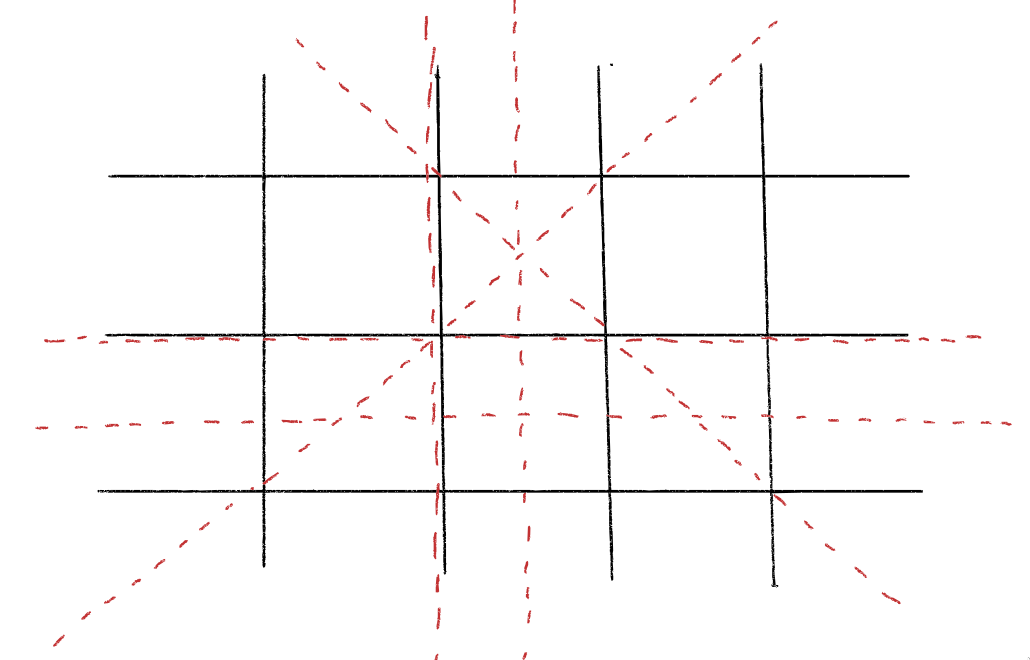
\includegraphics[width=0.6\linewidth]{./res/Pics/3_1_b.png}
    \caption{}\label{fig:3-1-b}
  \end{figure}

  There are six mirror lines: one horizontal/vertical pair that aligns with the lattice sites, one on their midpoint, and a diagonal pair.


\item This one is in Fig.~\ref{fig:3-1-c-1}. The red dot corresponds to the six-fold rotation axis and the green to the three-fold axis.

  \begin{figure}[]
    \centering
    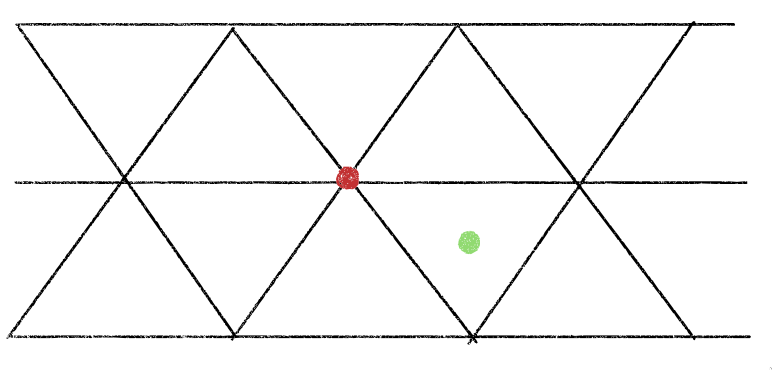
\includegraphics[width=0.45\linewidth]{./res/Pics/3_1_c_11.png}
    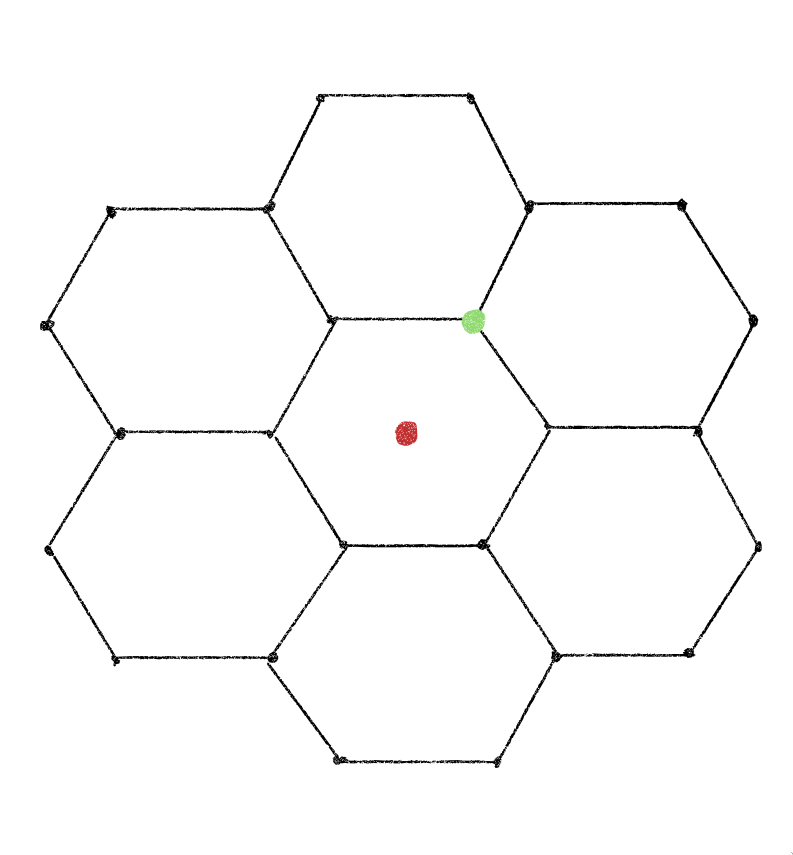
\includegraphics[width=0.45\linewidth]{./res/Pics/3_1_c_12.png}
    \caption{}\label{fig:3-1-c-1}
  \end{figure}

  \begin{figure}[]
    \centering
    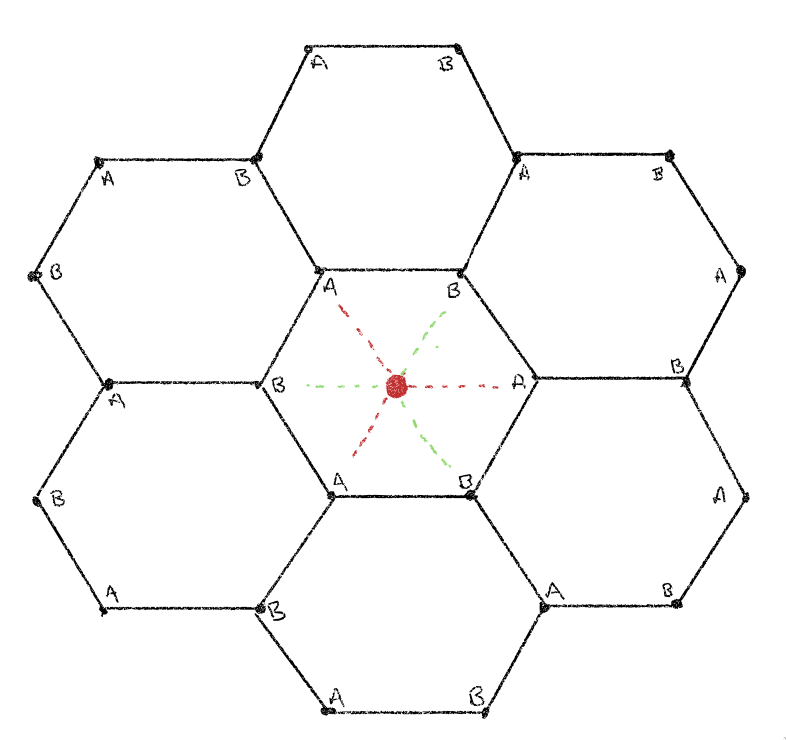
\includegraphics[width=0.6\linewidth]{./res/Pics/3_1_c_2.png}
    \caption{}\label{fig:3-1-c-2}
  \end{figure}

  In the case of the A and B sites not being identical (like I drew in Fig.~\ref{fig:3-1-c-2}), the six-fold rotation axis becomes the same as the three-fold rotation axis for a triangular lattice.


\item Let's say that we are in the center of a pentagonal unit cell, where we have five-fold rotational symmetry. We can consider one such lattice vector $\vv{R}_{\vv{n}}$ that points from the center to one of the lattice sites. If we rotate once by $2\pi/5$, we get another lattice vector, say $\vv{R}_{\vv{m}}$ by rotational symmetry that points at another lattice site. If we rotate again, i.e. by a total angle of $4\pi/5$, we have the same deal; call this vector $\vv{R}_{\vv{\ell}}$.

  \begin{figure}[]
    \centering
    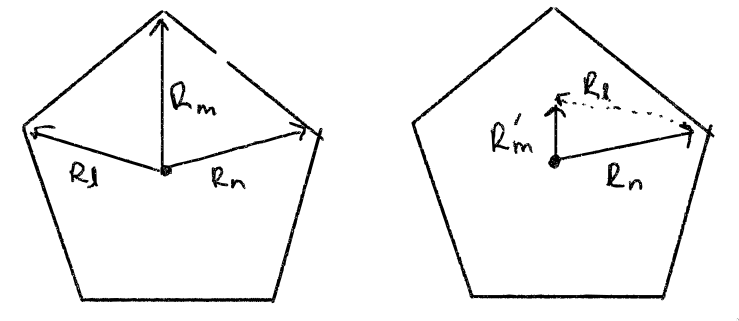
\includegraphics[width=0.6\linewidth]{./res/Pics/3-1-d.png}
    \caption{}\label{fig:3-1-d}
  \end{figure}

  Now, translational symmetry dictates that the sum of any two lattice vectors is itself a lattice vector. If we sum $\vv{R}_{\vv{n}}$ and $\vv{R}_{\vv{\ell}}$, we get a vector that is collinear with $\vv{R}_{\vv{m}}$, call it $\vv{R}_{\vv{m}'}$. I've done a little drawing in Fig.~\ref{fig:3-1-d}. However, we can easily tell that $\vv{R}_{\vv{m}'}$ is significantly shorter than $\vv{R}_{\vv{m}}$. We could begin to make the argument that, if it were to be \textit{longer}, it could point at another lattice site outside the unit cell, thus making it a valid lattice vector. However, this one resides entirely within this unit cell. By construction of this problem, the chosen lattice vectors and their rotated counterparts consitute the ``shortest paths'' to the 5 surrounding lattice sites from our rotation point. Therefore, in our case, $\vv{R}_{\vv{m}'}$ cannot be a lattice vector since it is shorter than any of the shortest paths to the lattice sites.
  
  Hence, translational symmetry is violated, meaning that five-fold rotational symmetry cannot co-exist with translational invariance.

  A rotation in 3D about an axis corresponds to the rotation of the (2D) plane perpendicular to the axis about a point in that plane. Since we know that five-fold rotational symmetry doesn't work in this 2D case, then by extension, it must also not work in the 3D case.

\end{parts}

%%% Local Variables:
%%% mode: LaTeX
%%% TeX-master: "../../HW3"
%%% End:
